\chapter{Introduction}
\section{Diffuse Optics}
The desire to use light to characterize human tissues and carry out tissue biopsy is pervasive in science-fiction has begun to penetrate the more traditional scientific and medical communities.  Early attempts to use light for tissue imaging, for example, date back to the 1930's when transillumination images of breast were used to detect the ``shadows" of tumors \cite{Cutler1931}. Unfortunately, because tissue is both highly absorbing and highly scattering, such crude light projections were found to be too unreliable for medical use, especially when compared to standard techniques in the clinic such as x-ray imaging. 

The potential for clinical imaging with light was revisited in the 1970's and 80's with the rediscovery of the so-called spectral ``window" in tissue \cite{Jobsis1977,Jo1999,Jo1999a}.  Indeed, light in the near-infrared (NIR) part of the spectrum ($600-1000~\rm{nm}$) is minimally absorbed by tissue hemoglobin and water (Figure~\ref{fig:NIRwin}), though it is substantially scattered by tissue organelles. This realization eventually gave birth to the field of NIR spectroscopy. Minimal absorption in this spectral ``window" permitted light to penetrate deeply into tissue and thereby provided optical access to information about tissue chromophores such as oxy-hemoglobin (Hb$\rm{O_2}$), deoxy-hemoglobin (Hb), lipid, and water ($\rm{H_2}$O). However, at the time, these methods were better characterized as qualitative rather than quantitative.
%
\begin{figure}[t]
\centering
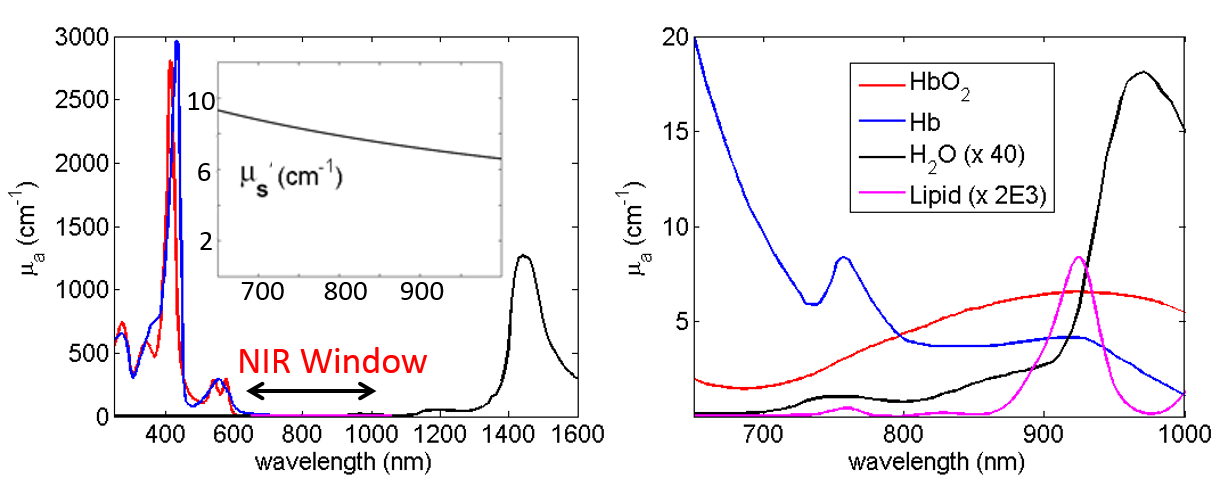
\includegraphics[width=14.5cm]{./figures/1_Introduction/NIRwin.png}
\caption[Spectra of the major chromophores in tissue showing the ``Near-infrared window"]{Spectra of the major chromophores in tissue showing the ``Near-infrared window". $\rm{H_2O}$ ($\times 40$) and lipid ($\times 2000$) has been scaled up to be visible on the plots. Hemoglobin concentrations for $150$g Hb/L (whole blood). a) Low absorption region that defines the NIR window; Inset: Estimated $\musp$ for breast tissues from Mie scattering theory in the NIR window. b) Tissue absorption coefficients in the NIR window for common chromophores. \textit{Spectral data compiled at http://omlc.org/spectra/index.html}}
\label{fig:NIRwin}
\end{figure}

The situation changed in the late 1980's and early 1990's when the community recognized that near-infrared (NIR) light diffuses in tissues \cite{Ishimaru1978,Rossum1999,Case1967}. In the diffusion model, photons travel along random walk trajectories through tissue. These light trajectories are characterized by a wavelength-dependent reduced scattering coefficient ($\musp(\lambda)$) (see Figure~\ref{fig:NIRwin} and Figure~\ref{fig:diffusephoto}), which is the reciprocal of the random walk step length, and a wavelength-dependent absorption coefficient ($\mua(\lambda)$), which depends on the concentrations of tissue chromophores such as oxy-hemoglobin (Hb$\rm{O_2}$), deoxy-hemoglobin (Hb), lipid, and water ($\rm{H_2}$O). Adoption of the diffusion model for light transport, in turn, opened up the possibility for quantitative diffuse optical spectroscopy (DOS) or near-infrared spectroscopy (NIRS). \cite{Boas1994,OLeary1996,McBride1999,Shah2001,Ntziachristos2002,Boas2002,Lin2002,Culver2003a,Cuccia2003,Yu2003,Merritt2003,Boas2004,Durduran2004,Shah2004,Jakubowski2004,Shah2005,Cerussi2006,Bassi2007,Cerussi2007,Xu2007,Franceschini2007,Zaman2007,Chung2008,Tseng2008,Jiang2009} and diffuse optical tomography (DOT) \cite{OLeary1995,Arridge1998a,Arridge1999,Siegel1999,Colak1999,Ntziachristos2000,Hawrysz2000,McBride2001,Pogue2001,Ntziachristos2002,Durduran2002,Intes2003,Culver2003,Corlu2003,Durduran2005,Choe2005a,Yates2005,Corlu2007,Lasker2007,Yalavarthy2007,Konecky2008a,Choe2009,Durduran2010,Flexman2011}. 
\begin{figure}[t]
\centering
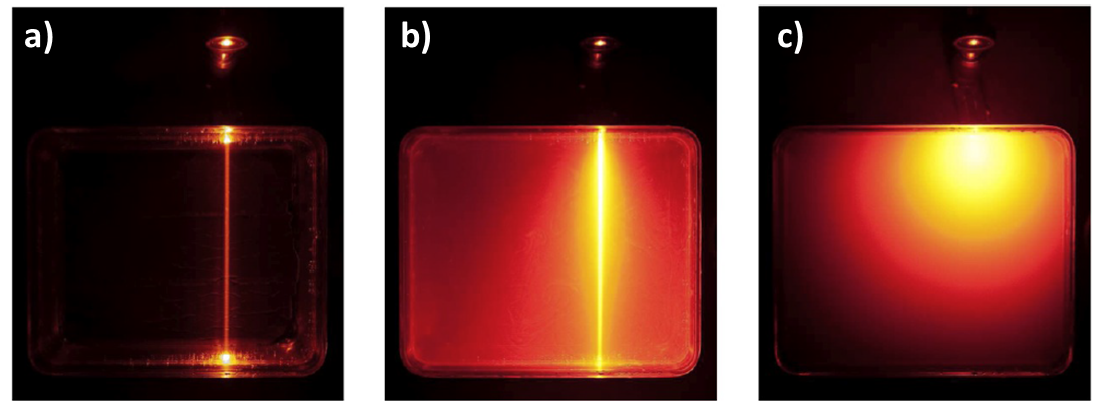
\includegraphics[width=14.5cm]{./figures/1_Introduction/diffusephoto.png}
\caption[Photo of light in varied scattering media]{Photograph showing a top-view image of a collimated NIR light beam as it passes through solutions with variable scattering coefficient ($\musp$). a) Small scattering coefficient. b) Medium scattering coefficient. c) Large scattering coefficient.}
\label{fig:diffusephoto}
\end{figure}

Of course, the key attraction of diffuse optical techniques is that they are sensitive to functional information about tissue hemodynamics and oxygen metabolism, e.g., as reflected in the variation of total hemoglobin concentration (THC), blood oxygen saturation (St$\rm{O_2}$), tissue scattering ($\musp$), and even tissue blood flow \cite{Culver2003a,Culver2003b,Durduran2004,Durduran2004b,Durduran2005,Yu2005,Yu2005a,Sunar2006,Zhou2006,Yu2007,Zhou2007,Carp2010,Kim2010,Shang2010,Diop2011,Irwin2011,Li2013,Durduran2014}. Indeed, all of these physiological parameters are pathologically relevant biomarkers of cancer, stroke, and other tissue disease/injury. Further, the diffuse optical methods have other attractive features. They are generally non-invasive, use non-ionizing radiation, are relatively rapid and portable, and they offer high-throughput (e.g., repeated or continuous measurements at the bedside). Finally, optical methods hold potential for use in multi-modal settings with other medical diagnostics such as ultrasound, MRI, X-ray, and PET.

In this thesis, I employ diffuse optics for imaging oxy- and deoxy-hemoglobin and tissue scattering in the human breast. My long-range goal is to use the contrast offered by these physiological parameters to identify and characterize breast lesions and to monitor breast tumor progression. This work builds on previous research in diffuse optical tomography, but it pushes the current limits of breast DOT both instrumentally and algorithmically. It is my hope that this research takes useful steps for clinical translation of quantitative DOT for breast cancer imaging.

\section{Spectroscopic monitoring and imaging of breast cancer}
For women in the U.S., breast cancer is the second most commonly diagnosed cancer (after skin cancer) and the second leading cause of cancer death (after lung cancer) \cite{Ma2013}.  While the mortality rate of breast cancer has decreased significantly in recent years, the overall number of women affected remains large. In $2012$, the American Cancer society estimated that $39,510$ of the $226,870$ new cases of breast cancer would lead to death in the U.S. \cite{Jemal2010}. In addition, the National Cancer Institute estimated the cost of breast cancer to the U.S. economy as greater than $\$8$ billion (2007) \cite{Barron2008}. 

Currently, many imaging modalities are in use for the detection, diagnosis and management of breast cancer. X-ray mammography is the most prevalent and widely adopted breast cancer screening tool; it employs ionizing photons to create high resolution projection images ($\sim0.1~\rm{mm}$/pixel). Ultrasound imaging is another useful method that probes the acoustic/mechanical properties of tissue with high-frequency sound waves; e.g., it uses acoustic wave reflection to locate a suspicious mass. Single Photon Emission Computed Tomography (SPECT) and Positron Emission Tomography (PET) represent still other useful imaging modalities based on the detection of gamma rays emitted from radioactive tagged proteins or sugars that are injected (or inhaled); tracking these macromolecules permits exploration of tissue metabolic pathways which can be different in tumors compared to normal tissues. Finally, Magnetic Resonance Imaging (MRI) employs radio waves and strong magnetic fields to probe tissue structure and function; these techniques rely on measurement of spin relaxation times to gain sensitivity to tissue micro-environment and to diagnose disease. 

All of these techniques have advantages (e.g., x-ray: high resolution, ultrasound: low cost, PET: metabolism detection, MRI: function and structure) and disadvantages (e.g., x-ray: ionizing radiation, ultrasound: contrast and penetration, PET: ionizing radiation, MRI: throughput and cost) that lead to arguments about which modality should be standard in breast cancer screening and diagnosis. In reality, no technology is perfect for all scenarios, and most modern approaches to breast cancer treatment utilize a combination of imaging technologies in synchrony with an array of treatments tailored to the patient (e.g., neoadjuvant chemotherapy, lumpectomy, mastectomy). In this environment, there is a need for additional modalities to detect cancers earlier, to detect cancers in populations with low specificity (e.g., women with dense breasts), and to track functional information during treatment (such as neoadjuvant chemotherapy).

By comparison to the medical diagnostics described above, diffuse optics is new. It also has different contrast mechanisms and complementary strengths. For example, DOT's ability to measure endogenous tissue chromophores (Hb, HbO) and exogenous optical contrast agents (ICG) provides access to functional processes and to parameters which are useful for detection and characterization of breast tumors with high sensitivity and specificity \cite{Zhao2015,Choe2009}. Cancer cells are accompanied by various growth factors that spur angiogenesis and can result in higher blood concentration in the tumor region \cite{Weidner1992,Thomsen1998,Zhu2003}; this variation in hemoglobin content can be detected as an absorption contrast optically. Further, cellular and extracelluar components, such as nuclei, mitochondia, and other organelles, are known to scatter light due to their refractive index differences and size, and their scattering can be modeled with Mie scattering theory \cite{Flock1987,Thomsen1990}. In tumors, these regions of enhanced cell growth and mitochondrial density can produce greater scattering compared to healthy tissue, and these scattering changes can be detected optically (see Figure~\ref{fig:cancercells}).
\begin{figure}[t]
\centering
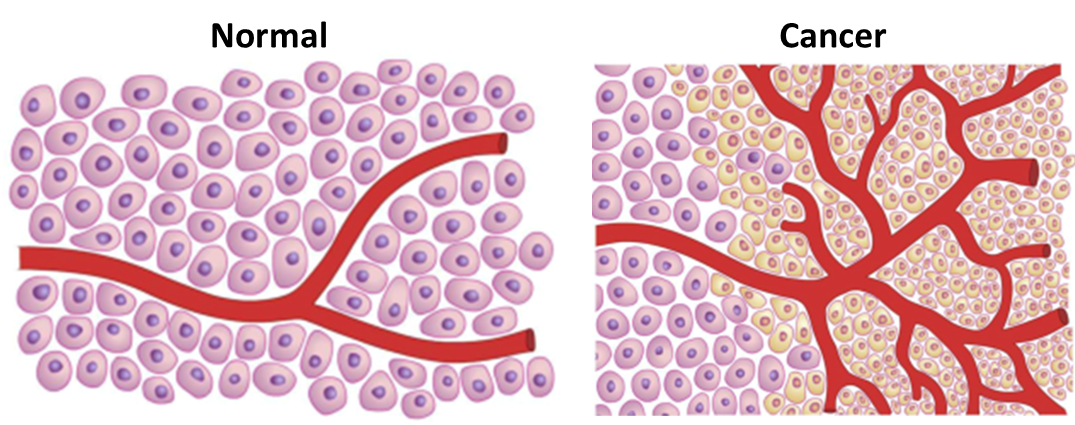
\includegraphics[width=14cm]{./figures/1_Introduction/cancercells.png}
\caption[Illustration of normal and cancer tissue]{Illustration of normal and cancer tissue. Cancer tissue regions have greater blood vessel and cell/cell-organelle densities due to angiogenesis and cell growth which can be differentiated optically compared to surrounding health tissue region. \textit{Figure courtesy of R. Choe.}\cite{Choe2005}}
\label{fig:cancercells}
\end{figure}

Further, as noted above, DOT is non-invasive, uses non-ionizing radiation, and is relatively low in cost compared to most diagnostic modalities, though it suffers from issues of low spatial resolution. Despite this apparent disadvantage, several groups (including ours) have shown that changes in optics-based physiological contrast can be utilized to distinguish between healthy and diseased tissue; this general approach has by now found use in investigations of muscle\cite{Chance1988,Lin2002,Yu2005a,Yu2007}, brain \cite{Gratton1990,Benaron1994,Houten1996,Boas2002,Hebden2002,Culver2003b,Culver2003a,Hebden2003,Siegel2003,Xu2003,Boas2004,Durduran2004,Choe2005,Zhou2006,Franceschini2007,Kim2010,Roche-Labarbe2010} and breast cancer. DOT, with its access to functional information, low cost, high throughput (of patients), and potentially high specificity and sensitivity is an attractive modality for development in the current roster of imaging technologies used in breast cancer diagnosis and treatment.

In the context of breast imaging, DOT utilizes light sources on the surface of tissues to illuminate the breast and employs detectors to access light that has been transmitted and scattered in tissue. With literally many thousands of source-detector pairs on the tissue boundaries, DOT readily employs these measured light fluence rate signals in order to computationally reconstruct the 3D distribution of $\mua$ and $\musp$ within the sampled tissue. While large DOT datasets have been prohibitively data intensive in the past, decreasing computational costs and increasing computational processing power make DOT a more attractive modality for clinical development. To date, DOT has successfully imaged tumors in the breast in a variety of clinical situations. For example it has been shown that DOT can differentiate of malignant and benign tumors \cite{McBride1999,Pogue2001,Ntziachristos2002,Leff2008,Tromberg2008,Choe2009,Wang2010}. DOT and DOS have also been shown to have potential for statistical separation of responders from partial responders to inform chemotherapy treatments \cite{Tromberg2005,Zhu2008,Schegerin2009,Jiang2009,Cerussi2011,Choe2012,Busch2013}. These studies point to DOT as a strong candidate for diagnosis and monitoring in modern breast cancer treatments and regiments that are targeted and unique to patients.

%
\section{Diffuse Optical Tomography instrumentation}
Presently, a few groups are exploring DOT, and as of yet no consensus of its best implementation has come about. Part of the problem is that DOT is quite flexible in its possible configurations, and each configuration has its own set of advantages and disadvantages. Typically, DOT systems vary in number of wavelengths used, number and arrangement of source-detector pairs, detection techniques, and, of course, algorithmic approaches.

Multi-spectral systems permit robust imaging of multiple chromophores, in part because \textit{a priori} spectral information about each chromophore exists and can be utilized. Many DOS and DOT systems will employ at least two wavelengths, but the best systems employ more wavelength which generally permit the quantification of more chromophores. Source-detector arrangements vary too. Most employ either the remission or transmission geometry. In the remission geometry, the source and detector are on the same side of the tissue surface; this configuration offers a great deal of flexibility and ease of measurement. Many remission systems, in fact, are handheld, and the optical properties of tissue located just below the probe are mapped out as the device is placed at several locations on the breast surface. One disadvantage of this geometry, however, is that the sensitivity function is depth-dependent, and the data are distorted to varying degrees with depth. Also, it is hard to penetrate too deeply in this geometry (e.g., the typical penetration is approximately one-half of the source-detector separation on the surface). In the transmission geometry, typical DOT source-detector arrangements include the ring~\cite{Pogue1995,Nioka1997,Poplack2007,Enfield2007} and the slab~\cite{Grosenick2005,Pifferi2003,Choe2009}. In general, transmission measurements provide much better sensitivity for deep tissues, since the detected light in this geometry is more likely to travel through all areas of interest.
\begin{figure}[t]
\centering
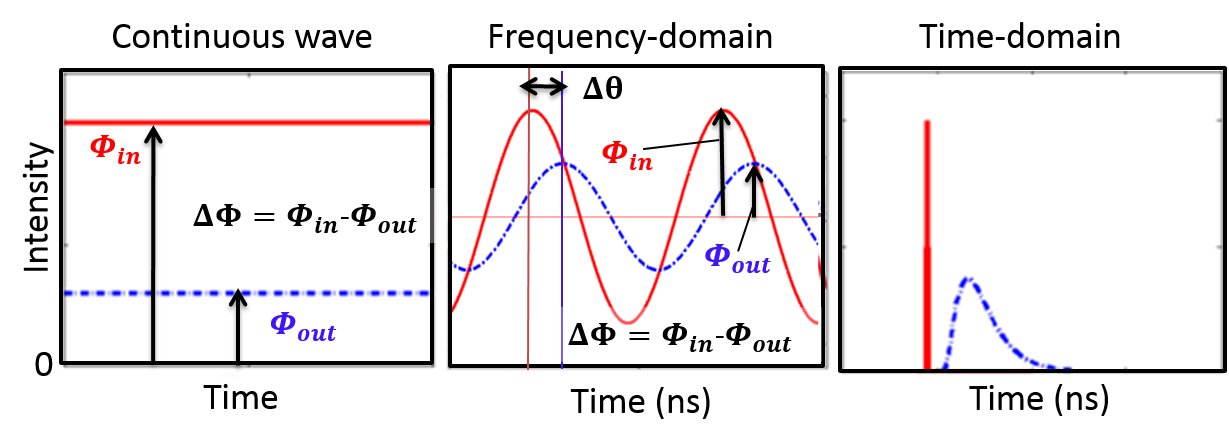
\includegraphics[width=14.5cm]{./figures/1_Introduction/detscheme.png}
\caption[Schematic illustration of the three optical data types used in diffuse optics]{Schematic illustration of the three optical data types used in diffuse optical experiments. The input signal is colored red and the output (detected) signal is colored blue. Continuous wave (CW) techniques measure the change in fluence rate amplitude $\Delta\Phi$. The frequency-domain (FD) methods amplitude modulate the light sources and measure both $\Delta\Phi$ and the phase shift, $\Delta\theta$, between the input and output waveforms. The time-domain (TD) technique measures to amplitude and broadening of a very short incident pulse as it travels through the medium; TD methods can be thought of as a superposition of FD measurements with many modulation frequencies.}
\label{fig:detscheme}
\end{figure}

These systems can be further divided by data-type, a property which also defines the experimental detection system and the nature of the experimental light sources. These data-types generally fall into three categories: continuous-wave (CW), frequency-domain (FD), and time domain (TD) (Figure~\ref{fig:detscheme}). CW systems are the most simple; in this case the variation in light amplitude (fluence-rate amplitude) is measured.  However, in these systems, the cross-talk between absorption and scattering is often severe; the cross-talk can be ameliorated via multi-spectral techniques \cite{Corlu2003,Corlu2005}, but the situation is definitely not perfect! Frequency-domain systems employ laser light sources that are intensity modulated (typically in the 50 MHz to GHz range); in this scenario, a diffusive wave is injected into the tissue with amplitude and phase that evolve as the light travels through the turbid medium. By measuring the amplitude and phase of the output signal (e.g., as a function of position, modulation frequency, etc.), one can rigorously separate absorption \textit{from} scattering contrasts. The FD detection scheme can be either homodyne or heterodyne. The data-types used in this thesis are either CW or FD. Time-domain (TD) systems use pulsed laser sources that inject short light pulses ($\leq $ps) into the turbid medium; these pulses broaden as they travel through the medium due to the different photon trajectories, and their broadening is measured by sophisticated time-correlated photon counting detection systems. Like FD systems, the TD methods also permit separation of scattering from absorption. The TD and FD experiments are essentially Fourier analogs. Numerous arguments have arisen in the community about whether TD is superior to FD or vice versa; these questions are still not resolved. Many factors come into play in analyzing these questions, ranging from duty cycle for best signal-to-noise, to detection systematic errors, to cost. 

\section{Diffuse Optical Tomography of Breast Cancer at Penn}
DOT and, more generally, diffuse optics has had a long history at Penn. For example, the first experimental tomographic reconstructions of absorption and scattering heterogeneities were demonstrated at Penn \cite{OLeary1995}; similarly the first fluorescent lifetime tomography with diffuse optics was carried out here \cite{OLeary1996}, as was the first fluorescence breast cancer imaging in humans \cite{Corlu2007}. In a different vein, numerous comparison and validation studies of DOT and other imaging modalities were performed here, including with PET \cite{Konecky2008b} and MRI \cite{Choe2005a}. Further, instruments have been developed that combine DOT with other modalities such as ultrasound \cite{Zhu1999,Holboke2000} and MRI \cite{Ntziachristos1999, Ntziachristos2000,Ntziachristos2001,Ntziachristos2002}; this approach enhances the ability of optics to extract functional information about tissues by using structural information provided by other techniques to constrain the inverse problem. 

Parallel to this experimental work, our group has developed theoretical approaches for DOT, including important research that shed light on the use and value of multiple optical wavelengths (and the optimization of the wavelength choice) for clinical DOT and DOS devices \cite{Corlu2003,Corlu2005}. Experiments characterizing (and pushing) the resolution of stand-alone DOT imaging were carried out \cite{Konecky2008a}, and a clinical DOT breast imaging device (Gen2) was built and used in a 47 patient study; the latter study demonstrated statistically significant differences in DOT contrast between malignant and benign lesions \cite{Choe2009}. From this research, we have learned that it is possible to use optical imaging as a clinical and a research tool to advance our understanding of breast cancer physiology and treatment.

In my thesis I present my work to build on this previous success at Penn, i.e., my work pushes the frontier further in order to translate DOT into the clinical setting. Specifically, I explored and addressed clinically relevant issues for DOT imaging such as the effect of the chest wall, and I designed and built the next generation DOT breast imaging device. This new instrument will advance the clinical application of DOT in terms of resolution and image fidelity (i.e., due substantially to the enormous amount of data obtainable from the new instrumentation and signal normalization/calibration in-situ), information content (i.e., due to separation of absorption and scattering contrast with frequency-domain detection), and overall image quality (i.e., due to improved patient interfaces, etc.). Finally, I have begun to reconstruct images using the instrument in tissue phantoms and in the clinic.

\section{Thesis Organization}
The remainder of this thesis is organized as follows. In Chapter 2, I review the underlying theory of diffuse light propagation in tissue, as well as selected image reconstruction techniques (especially ones that I employ for my experiments). Specifically, I derive analytical solutions in frequency domain for the geometries and boundary conditions commonly used in diffuse optical tomography. I also describe the linear and nonlinear methods used to solve the forward and inverse problems that are utilized in my experimental image reconstructions.

Chapter 3 describes a (published) benchtop experiment wherein I systematically explore diffuse optical tomography in the clinically relevant slab geometry in the presence of the chest wall. The effect that the chest wall has on DOT reconstructions is not understood. The chest is highly absorptive tissue that breaks the symmetry of the inverse problem, among other things. DOT reconstruction methods have not been systematically studied in this important regime. The use of a high spatial-density of source-detector pairs helps us to characterize the resulting systematics and also enables us to explore various schemes to mitigate these chest wall effects.

Chapter 4 introduces, explains, and characterizes the new Gen3 breast imaging instrument; then I describe first imaging tests with the instrument. These first experiments are deployed in the lab (with tissue phantoms) and then in the clinic. Details of the optics, electronics, detection are provided in Section \ref{sec:Gen3}. Details of the data processing and signal correction/normalization are discussed in Section \ref{sec:gen3pp}. The design, construction, and testing of this instrument is the most important research in this thesis. The image reconstruction research takes the first of many steps towards clinical DOT investigations, and teaches us about important issues in image regularization with DOT.  Data and image reconstructions from simulation and tissue phantom experiments highlight the multi-spectral and frequency-domain capabilities of the device. Finally, the first clinical image reconstructions from cancer patients are shown; with these first images, I establish that more work is needed to find the best algorithms for the apparatus, but the work helps to define these new directions for research. Chapter 5 summarizes my work and offers suggestions for further development of the research.
